% This is "sig-alternate.tex" V2.1 April 2013
% This file should be compiled with V2.5 of "sig-alternate.cls" May 2012
%
% This example file demonstrates the use of the 'sig-alternate.cls'
% V2.5 LaTeX2e document class file. It is for those submitting
% articles to ACM Conference Proceedings WHO DO NOT WISH TO
% STRICTLY ADHERE TO THE SIGS (PUBS-BOARD-ENDORSED) STYLE.
% The 'sig-alternate.cls' file will produce a similar-looking,
% albeit, 'tighter' paper resulting in, invariably, fewer pages.
%
% ----------------------------------------------------------------------------------------------------------------
% This .tex file (and associated .cls V2.5) produces:
%       1) The Permission Statement
%       2) The Conference (location) Info information
%       3) The Copyright Line with ACM data
%       4) NO page numbers
%
% as against the acm_proc_article-sp.cls file which
% DOES NOT produce 1) thru' 3) above.
%
% Using 'sig-alternate.cls' you have control, however, from within
% the source .tex file, over both the CopyrightYear
% (defaulted to 200X) and the ACM Copyright Data
% (defaulted to X-XXXXX-XX-X/XX/XX).
% e.g.
% \CopyrightYear{2007} will cause 2007 to appear in the copyright line.
% \crdata{0-12345-67-8/90/12} will cause 0-12345-67-8/90/12 to appear in the copyright line.
%
% ---------------------------------------------------------------------------------------------------------------
% This .tex source is an example which *does* use
% the .bib file (from which the .bbl file % is produced).
% REMEMBER HOWEVER: After having produced the .bbl file,
% and prior to final submission, you *NEED* to 'insert'
% your .bbl file into your source .tex file so as to provide
% ONE 'self-contained' source file.
%
% ================= IF YOU HAVE QUESTIONS =======================
% Questions regarding the SIGS styles, SIGS policies and
% procedures, Conferences etc. should be sent to
% Adrienne Griscti (griscti@acm.org)
%
% Technical questions _only_ to
% Gerald Murray (murray@hq.acm.org)
% ===============================================================
%
% For tracking purposes - this is V2.0 - May 2012

\documentclass{sig-alternate-05-2015}

\usepackage{tikz}
\usetikzlibrary{arrows,positioning,automata}
\usepackage[noend]{algpseudocode}
\usepackage{algorithm}
\usepackage{enumitem, kantlipsum}

% Use the postscript times font!
\usepackage{times}

\usepackage{mathtools}
\usepackage{amssymb}

\begin{document}

% Copyright
\setcopyright{acmcopyright}
%\setcopyright{acmlicensed}
%\setcopyright{rightsretained}
%\setcopyright{usgov}
%\setcopyright{usgovmixed}
%\setcopyright{cagov}
%\setcopyright{cagovmixed}


% DOI
\doi{10.475/123_4}

% ISBN
\isbn{123-4567-24-567/08/06}

%Conference
\conferenceinfo{PLDI '13}{June 16--19, 2013, Seattle, WA, USA}

\acmPrice{\$15.00}

%
% --- Author Metadata here ---
\conferenceinfo{WOODSTOCK}{'97 El Paso, Texas USA}
%\CopyrightYear{2007} % Allows default copyright year (20XX) to be over-ridden - IF NEED BE.
%\crdata{0-12345-67-8/90/01}  % Allows default copyright data (0-89791-88-6/97/05) to be over-ridden - IF NEED BE.
% --- End of Author Metadata ---

\title{Human-Robot Collaboration}
% \subtitle{[Extended Abstract]
%
% You need the command \numberofauthors to handle the 'placement
% and alignment' of the authors beneath the title.
%
% For aesthetic reasons, we recommend 'three authors at a time'
% i.e. three 'name/affiliation blocks' be placed beneath the title.
%
% NOTE: You are NOT restricted in how many 'rows' of
% "name/affiliations" may appear. We just ask that you restrict
% the number of 'columns' to three.
%
% Because of the available 'opening page real-estate'
% we ask you to refrain from putting more than six authors
% (two rows with three columns) beneath the article title.
% More than six makes the first-page appear very cluttered indeed.
%
% Use the \alignauthor commands to handle the names
% and affiliations for an 'aesthetic maximum' of six authors.
% Add names, affiliations, addresses for
% the seventh etc. author(s) as the argument for the
% \additionalauthors command.
% These 'additional authors' will be output/set for you
% without further effort on your part as the last section in
% the body of your article BEFORE References or any Appendices.

\numberofauthors{8} %  in this sample file, there are a *total*
% of EIGHT authors. SIX appear on the 'first-page' (for formatting
% reasons) and the remaining two appear in the \additionalauthors section.
%
\author{
% You can go ahead and credit any number of authors here,
% e.g. one 'row of three' or two rows (consisting of one row of three
% and a second row of one, two or three).
%
% The command \alignauthor (no curly braces needed) should
% precede each author name, affiliation/snail-mail address and
% e-mail address. Additionally, tag each line of
% affiliation/address with \affaddr, and tag the
% e-mail address with \email.
%
% 1st. author
\alignauthor
Mahni Shayganfar \\
       \affaddr{Worcester Polytechnic Institute}\\
       \affaddr{100 Institute Road}\\
       \affaddr{Worcester, MA 01609}\\
       \email{mshayganfar@wpi.edu}
% 2nd. author
\alignauthor
Charles Rich \\
       \affaddr{Worcester Polytechnic Institute}\\
       \affaddr{100 Institute Road}\\
       \affaddr{Worcester, MA 01609}\\
       \email{rich@wpi.edu}
\and
% 3rd. author
\alignauthor 
Candace L. Sidner\\
       \affaddr{Worcester Polytechnic Institute}\\
       \affaddr{100 Institute Road}\\
       \affaddr{Worcester, MA 01609}\\
       \email{sidner@wpi.edu}
% 4th. author
\alignauthor 
Benjamin L. Hyl\'ak\\
       \affaddr{Worcester Polytechnic Institute}\\
       \affaddr{100 Institute Road}\\
       \affaddr{Worcester, MA 01609}\\
       \email{blhylak@wpi.edu}
}
% There's nothing stopping you putting the seventh, eighth, etc.
% author on the opening page (as the 'third row') but we ask,
% for aesthetic reasons that you place these 'additional authors'
% in the \additional authors block, viz.
\additionalauthors{Additional authors: John Smith (The Th{\o}rv{\"a}ld Group,
email: {\texttt{jsmith@affiliation.org}}) and Julius P.~Kumquat
(The Kumquat Consortium, email: {\texttt{jpkumquat@consortium.net}}).}
\date{30 July 1999}
% Just remember to make sure that the TOTAL number of authors
% is the number that will appear on the first page PLUS the
% number that will appear in the \additionalauthors section.

\maketitle
\begin{abstract}
We have investigated the mutual influences of affective and collaborative
processes in a cognitive theory to support interaction between humans and robots
or virtual agents. We build primarily on the \textit{cognitive appraisal} theory of
emotions and the \textit{SharedPlans} theory of collaboration to investigate the
structure, fundamental processes and functions of emotions in a collaboration.
We have developed new algorithms for appraisal processes as part of a new
overall computational model. We have evaluated our implemented algorithms by
conducting an online user study.
\end{abstract}


%
% The code below should be generated by the tool at
% http://dl.acm.org/ccs.cfm
% Please copy and paste the code instead of the example below. 
%
\begin{CCSXML}
<ccs2012>
 <concept>
  <concept_id>10010520.10010553.10010562</concept_id>
  <concept_desc>Computer systems organization~Embedded systems</concept_desc>
  <concept_significance>500</concept_significance>
 </concept>
 <concept>
  <concept_id>10010520.10010575.10010755</concept_id>
  <concept_desc>Computer systems organization~Redundancy</concept_desc>
  <concept_significance>300</concept_significance>
 </concept>
 <concept>
  <concept_id>10010520.10010553.10010554</concept_id>
  <concept_desc>Computer systems organization~Robotics</concept_desc>
  <concept_significance>100</concept_significance>
 </concept>
 <concept>
  <concept_id>10003033.10003083.10003095</concept_id>
  <concept_desc>Networks~Network reliability</concept_desc>
  <concept_significance>100</concept_significance>
 </concept>
</ccs2012>  
\end{CCSXML}

\ccsdesc[500]{Computer systems organization~Embedded systems}
\ccsdesc[300]{Computer systems organization~Redundancy}
\ccsdesc{Computer systems organization~Robotics}
\ccsdesc[100]{Networks~Network reliability}


%
% End generated code
%

%
%  Use this command to print the description
%
\printccsdesc

% We no longer use \terms command
%\terms{Theory}

\keywords{Human-Robot Collaboration, Affect-Driven Processes}



\begin{table*}
\centering
\caption{Some Typical Commands}
\begin{tabular}{|p{4.5cm}|p{10cm}|p{1.2cm}|} \hline
Question Category&Question&Question Number\\
\hline \texttt Likability&I would like to continue working with the
robot.&Q1\\
\hline \texttt Likability&I felt close to the robot.&Q2\\
\hline \texttt Trust&I trust the robot.&Q3\\
\hline \texttt Trust&I trust the robot to perform appropriately in our
collaboration.&Q4\\
\hline \texttt Robot's Performance&The robot was repetitive.&Q5\\
\hline \texttt Robot's Performance&The robot's decisions improved my
performance during the collaboration.&Q6\\
\hline \texttt Robot's Understanding - Human Emotions&The robot understood my
emotions.&Q7\\
\hline \texttt Robot's Understanding - Human Emotions&The robot understands
some of my feelings and takes them into account in our
collaboration.&Q8\\
\hline \texttt Robot's Understanding - Goals&The robot perceives
accurately what my objectives are.&Q9\\
\hline \texttt Robot's Understanding - Goals&The robot was
committed to the collaboration.&Q10\\
\hline \texttt Human Feeling - Collaboration&The robot and I are
working towards mutually agreed-upon goals.&Q11\\
\hline \texttt Human Feeling - Collaboration&I am satisfied
with the outcome of our collaboration.&Q12\\
\hline \texttt Satisfaction - Collaborative Partner&The robot was satisfied
with my collaborative behavior.&Q13\\
\hline \texttt Satisfaction - Collaborative Partner&I was satisfied with the
robot.&Q14\\
\end{tabular}
\end{table*}
% end the environment with {table*}, NOTE not {table}!

\begin{figure*}[tbh]
\centering
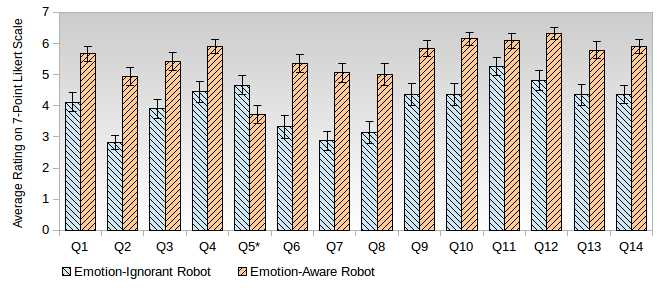
\includegraphics[width=\textwidth]{figure/14Questions.png}
\caption{A sample black and white graphic
that has been resized with the \texttt{includegraphics} command.}
\end{figure*}

 \begin{table*}
\centering
\caption{Some Typical Commands}
\begin{tabular}{|p{6.7cm}|p{3cm}|p{1.5cm}|p{3.2cm}|p{1.2cm}|} \hline
Question&No. Participants Favoring Emotion-Aware&Total No.
Participants&Percentage Participants Favoring Emotion-Aware&P-value\\
\hline \texttt Which of the two runs with the robot did you
prefer?&33&33&100&0\\
\hline \texttt In which of the two runs did the robot exhibit behavior that
could be useful in a more complex task?&30&32&93.75&\ll0.001\\
\hline \texttt In which of two runs did the robot exhibit behavior that could
prevent human error?&18&30&60&0.200\\
\hline \texttt In which of the two runs did the robot exhibit behavior that
could improve the efficiency of collaboration?&26&31&83.9&\ll0.001\\
\hline \texttt What was the most interesting behavior of the robot and in which
run did it happen?&24&29&82.8&\ll0.001\\
\end{tabular}
\end{table*}


\section{Experimental Scenario}

\subsection{The Robot}

\subsection{Interaction Paradigms}

\subsection{Environment and Tasks}



\section{Experimental Design}



\section{Experimental Scenario}



\section{Study Design and Procedure}

\subsection{Software Architecture}

\subsection{Robotic Implementation}




\section{Evaluation and Results}

\subsection{Hypothesis}

\subsection{Setting and Conditions}

\subsection{Procedure}

\subsection{Measurements}

\subsection{Evaluation Results}




\section{Analysis and Discussion}

\subsection{Emotion Ignorant Robot}

\subsection{Emotion A Robot}

\subsection{Generalization and Limitations}




\section{General Discussion}




\section{Conclusions}


%ACKNOWLEDGMENTS are optional
\section{Acknowledgments}

%
% The following two commands are all you need in the
% initial runs of your .tex file to
% produce the bibliography for the citations in your paper.
\bibliographystyle{abbrv}
\bibliography{mshayganfar}  % sigproc.bib is the name of the Bibliography in
% this case You must have a proper ".bib" file
%  and remember to run:
% latex bibtex latex latex
% to resolve all references
%
% ACM needs 'a single self-contained file'!
%
%APPENDICES are optional
%\balancecolumns
\end{document}
